\documentclass[11pt,a4paper]{article}

\usepackage{fontspec}
\setmainfont{Lato}

\usepackage[a4paper,margin=2cm,top=2.2cm,bottom=2.2cm]{geometry}
\usepackage{xcolor}
\usepackage{graphicx}
\usepackage[most]{tcolorbox}
\usepackage{enumitem}
\usepackage{titlesec}
\usepackage{fancyhdr}
\usepackage{hyperref}
\usepackage{tikz}

% ---- Paleta baseada no site (verde pinheiro, vermelho natalino, dourado) ----
\definecolor{pine}{HTML}{123B2A}
\definecolor{pinelight}{HTML}{1F5A3E}
\definecolor{cranberry}{HTML}{B3223A}
\definecolor{gold}{HTML}{D8A340}
\definecolor{cream}{HTML}{F4F1E9}
\definecolor{ink}{HTML}{1A1A1A}
\definecolor{graytxt}{HTML}{555555}

\pagecolor{white}
\color{ink}

% ---- Titulos de secao ----
\titleformat{\section}
  {\Large\bfseries\color{pine}}
  {}{0em}{}
\titlespacing*{\section}{0pt}{1.4em}{0.8em}

\titleformat{\subsection}
  {\large\bfseries\color{cranberry}}
  {}{0em}{}
\titlespacing*{\subsection}{0pt}{1.1em}{0.5em}

% ---- Cabecalho/rodape ----
\pagestyle{fancy}
\fancyhf{}
\renewcommand{\headrulewidth}{0pt}
\fancyfoot[C]{\small\color{graytxt} Geometria Natalina --- Alinhamento com a BNCC}
\fancyfoot[R]{\small\color{graytxt}\thepage}

% ---- Caixa de missao / destaque ----
\newtcolorbox{missionbox}{
  colback=cream, colframe=gold, boxrule=1pt, arc=3pt,
  left=10pt, right=10pt, top=8pt, bottom=8pt, breakable
}

\newtcolorbox{habilidade}[1]{
  colback=white, colframe=pine, boxrule=0.8pt, arc=2pt,
  left=10pt, right=10pt, top=7pt, bottom=7pt, breakable,
  title={#1}, coltitle=white, colbacktitle=pine, fonttitle=\bfseries
}

% ---- Figura com legenda estilizada ----
\newcommand{\shot}[3]{%
  \begin{center}
  \begin{tcolorbox}[colback=white, colframe=pine!60, boxrule=1pt, arc=3pt,
      left=4pt, right=4pt, top=4pt, bottom=4pt, breakable]
    \includegraphics[width=#2\linewidth]{#1}
  \end{tcolorbox}
  {\small\color{graytxt}\itshape #3}
  \end{center}
}

\setlist[itemize]{leftmargin=1.4em, itemsep=0.15em, topsep=0.3em}

\begin{document}

% ===================== CAPA =====================
\begin{titlepage}
\newgeometry{margin=0cm}
\noindent
\begin{tikzpicture}[remember picture, overlay]
  \fill[pine] (current page.north west) rectangle (current page.south east);
  \fill[cranberry] ([yshift=1cm]current page.south west) rectangle ([yshift=1.3cm]current page.south east);
  \node[anchor=north, text width=15cm, align=center] at ([yshift=-4.5cm]current page.north) {
    {\color{gold}\Large\bfseries JOGO EDUCACIONAL DIGITAL}
  };
  \node[anchor=center, text width=16cm, align=center] at (current page.center) {
    {\color{white}\fontsize{40}{46}\selectfont\bfseries Geometria Natalina}\\[0.6cm]
    {\color{cream}\Large Aprender geometria criando, explorando e jogando}
  };
  \node[anchor=south, text width=15cm, align=center] at ([yshift=2.2cm]current page.south) {
    {\color{white}\normalsize Alinhamento pedagógico com a Base Nacional Comum Curricular (BNCC)}
  };
\end{tikzpicture}
\end{titlepage}
\restoregeometry

% ===================== APRESENTACAO =====================
\section*{Apresentação}

\textbf{Geometria Natalina} é um jogo educacional digital que transforma conceitos de geometria em desafios visuais com temática natalina. O estudante percorre um \emph{caderno de desafios} e constrói desenhos em um plano cartesiano a partir de pontos e segmentos.

\shot{screenshots/dashboard.png}{0.8}{Tela inicial: caderno de desafios, progressão de XP e níveis.}

A proposta combina criatividade, raciocínio espacial e progressão gamificada. O aluno recebe experiência, avança de nível, desbloqueia desafios e acompanha suas tentativas e conquistas.

% ===================== COMO FUNCIONA =====================
\section*{Como funciona}

Cada desafio apresenta uma figura que pode ser construída por meio da identificação de pontos, segmentos e formas geométricas. O estudante precisa observar a representação, interpretar coordenadas e reproduzir a figura no plano cartesiano.

\shot{screenshots/desafio1.png}{0.8}{Desafio ``Presente'': o jogo indica a missão (marcar um ponto) e acompanha pontos e tentativas em tempo real.}

Os desafios trabalham diferentes ideias matemáticas:

\begin{itemize}
  \item pares ordenados e localização no plano;
  \item segmentos de reta e composição de figuras;
  \item polígonos e seus elementos;
  \item simetria;
  \item triângulos e quadriláteros;
  \item quadrantes do plano cartesiano;
  \item organização espacial e visualização geométrica.
\end{itemize}

\shot{../imagens-desenhos/1-presente.png}{0.55}{Figura-alvo do Desafio 1 --- Presente.}

% ===================== BNCC =====================
\section*{Relação com a BNCC}

As atividades podem ser articuladas principalmente às seguintes habilidades da BNCC de Matemática:

\begin{habilidade}{EF06MA18 --- Polígonos}
Reconhecer, nomear e comparar polígonos, considerando lados, vértices e ângulos, classificando-os em regulares e não regulares, tanto em representações no plano como em faces de poliedros.

\vspace{4pt}
No desafio do presente e na composição da árvore, o estudante identifica e combina quadriláteros, triângulos e outros polígonos para formar uma figura maior.
\end{habilidade}

\begin{habilidade}{EF06MA19 --- Triângulos}
Identificar características dos triângulos e classificá-los em relação às medidas dos lados e dos ângulos.

\vspace{4pt}
A árvore de Natal é composta por diferentes triângulos sobrepostos. A atividade pode estimular a comparação de seus lados, vértices e posições.
\end{habilidade}

\begin{habilidade}{EF06MA16 --- Plano cartesiano}
Associar pares ordenados a pontos do plano cartesiano do primeiro quadrante, em situações como a localização dos vértices de polígonos.

\vspace{4pt}
O jogo utiliza coordenadas para indicar onde cada ponto deve ser localizado. O aluno transforma pares ordenados em posições concretas no desenho.
\end{habilidade}

\begin{habilidade}{EF07MA21 --- Transformações geométricas}
Reconhecer e construir figuras obtidas por simetrias de translação, rotação e reflexão, usando instrumentos de desenho ou softwares de geometria dinâmica.

\vspace{4pt}
O desafio da estrela oferece uma oportunidade de explorar simetria e regularidade, observando como partes da figura se relacionam em torno de eixos e pontos de referência.
\end{habilidade}

% ===================== COMPETENCIAS =====================
\section*{Competências desenvolvidas}

Ao jogar, o estudante desenvolve a capacidade de:

\begin{itemize}
  \item interpretar representações geométricas;
  \item localizar pontos e estabelecer relações espaciais;
  \item reconhecer propriedades de figuras planas;
  \item analisar simetrias e padrões;
  \item planejar uma construção antes de executá-la;
  \item verificar erros e ajustar estratégias;
  \item comunicar seu raciocínio por meio de desenhos e coordenadas.
\end{itemize}

\begin{center}
\begin{tcolorbox}[colback=white, colframe=pine!60, boxrule=1pt, arc=3pt, left=4pt,right=4pt,top=4pt,bottom=4pt]
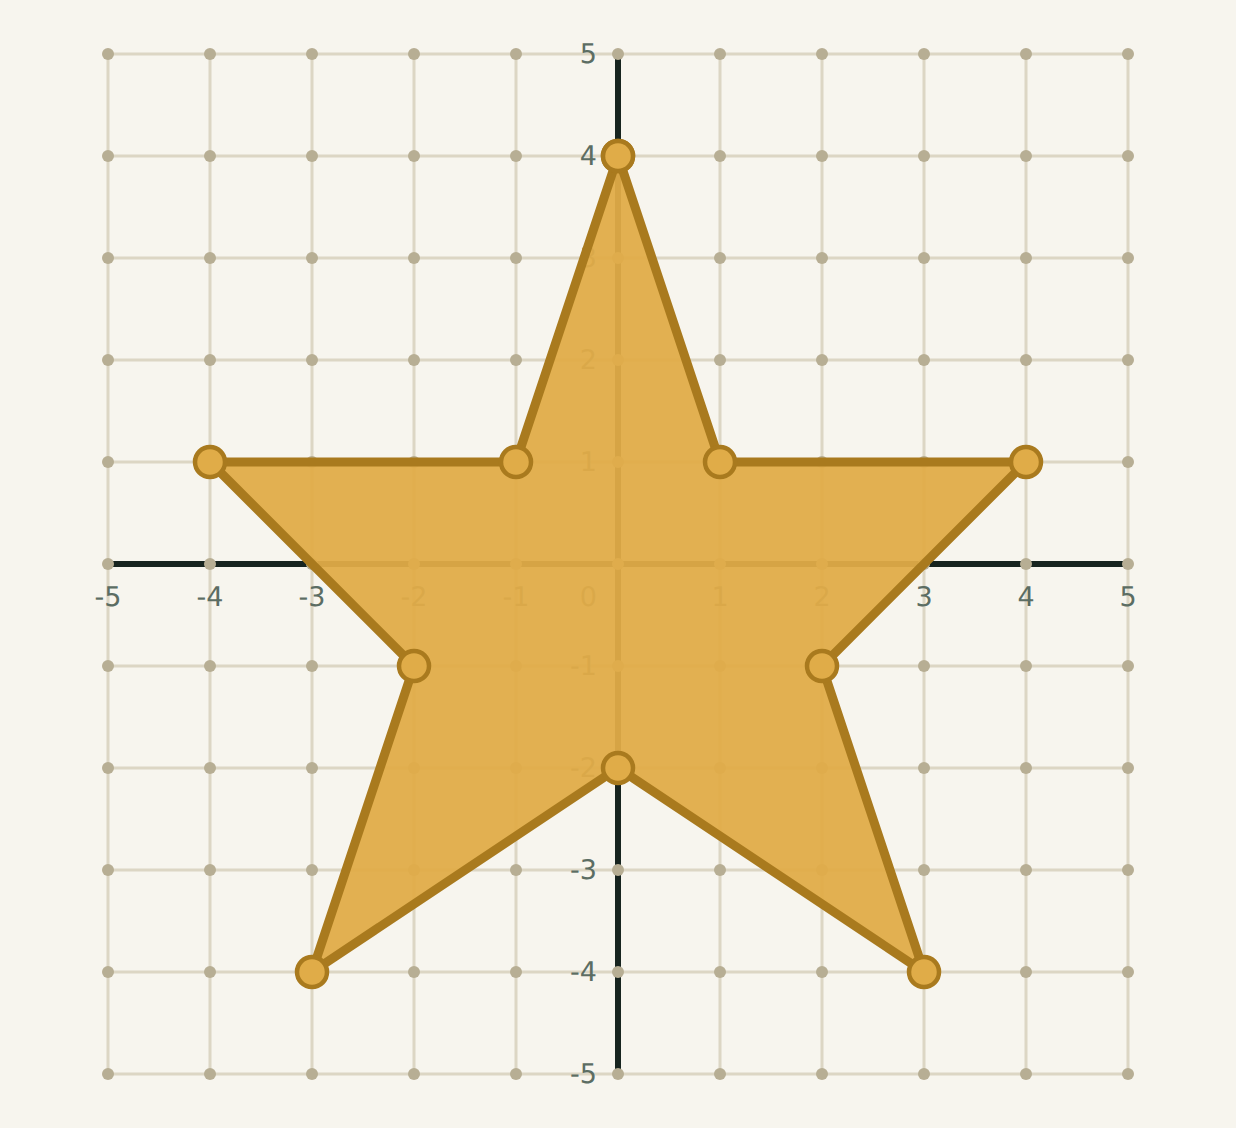
\includegraphics[width=0.4\linewidth]{../imagens-desenhos/2-estrela.png}
\hspace{0.5cm}
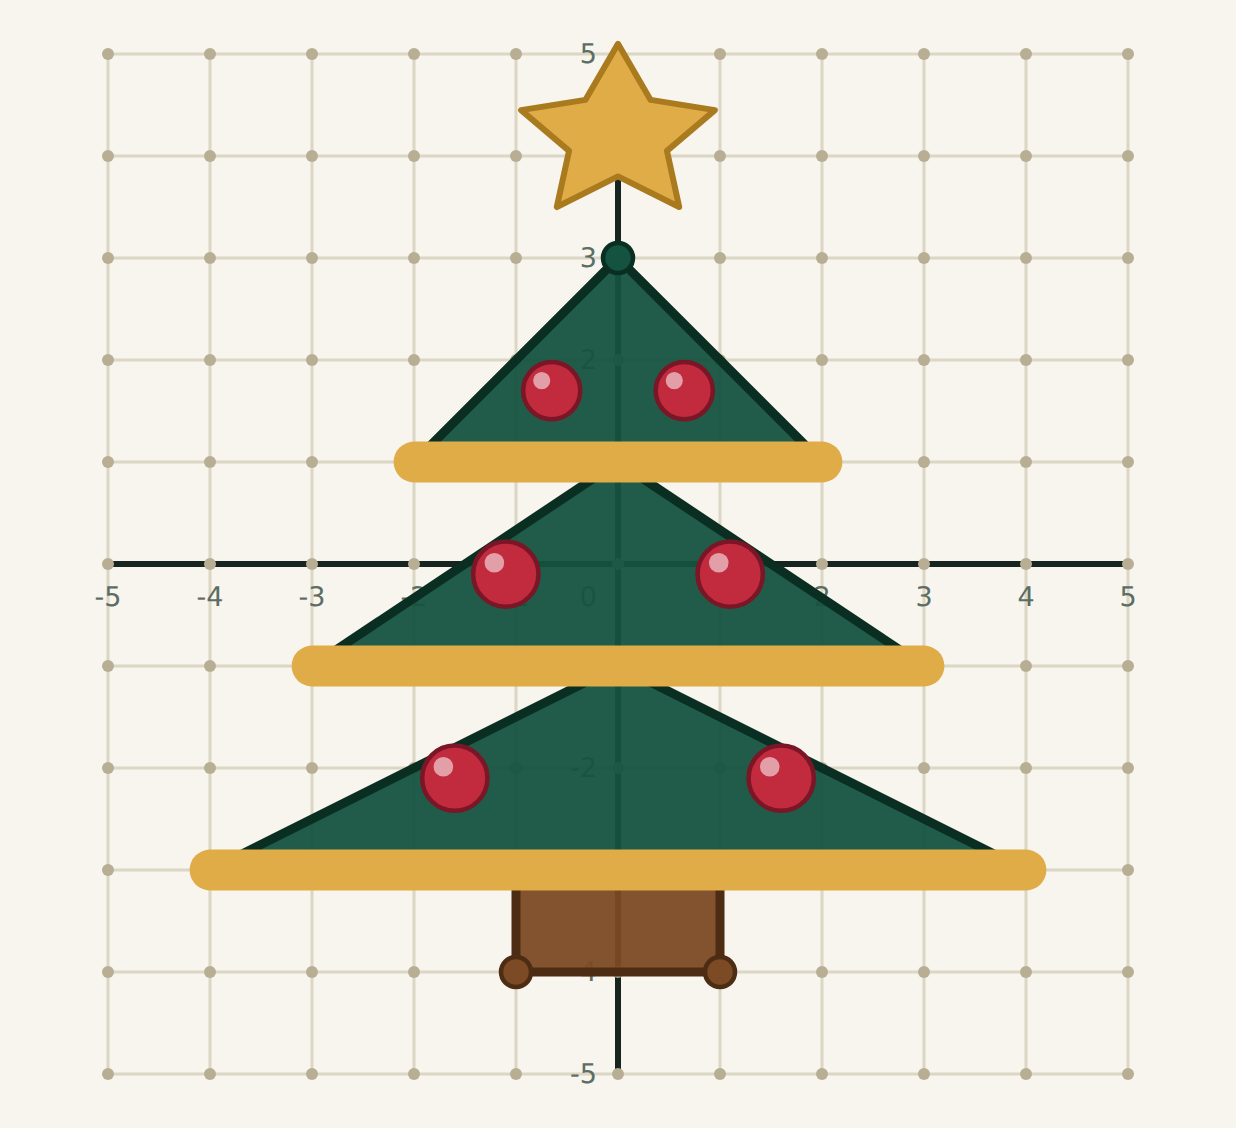
\includegraphics[width=0.4\linewidth]{../imagens-desenhos/3-arvore.png}
\end{tcolorbox}
{\small\color{graytxt}\itshape Figuras-alvo dos desafios 2 (Estrela) e 3 (Árvore de Natal).}
\end{center}

% ===================== GAMIFICACAO =====================
\section*{Gamificação e aprendizagem}

A progressão por níveis e desafios cria uma sequência de aprendizagem com objetivos claros. A experiência acumulada, os desafios desbloqueados e o registro de tentativas permitem que o aluno perceba sua evolução.

A temática natalina funciona como contexto motivador, aproximando a geometria de uma produção criativa. O estudante não apenas responde a perguntas: ele constrói presentes, estrelas e árvores usando conceitos matemáticos.

% ===================== POSSIBILIDADES =====================
\section*{Possibilidades pedagógicas}

O jogo pode ser utilizado como:

\begin{itemize}
  \item atividade de introdução ao plano cartesiano;
  \item prática de identificação de polígonos;
  \item revisão de vértices, lados e segmentos;
  \item exploração de simetria;
  \item atividade complementar em aulas de geometria;
  \item proposta de aprendizagem baseada em desafios;
  \item instrumento de avaliação formativa.
\end{itemize}

\begin{missionbox}
\textbf{Sugestão de uso em sala:} o professor pode propor que os alunos expliquem quais figuras aparecem em cada desenho, indiquem os pares ordenados utilizados, comparem os polígonos e criem novas figuras temáticas.
\end{missionbox}

% ===================== SINTESE =====================
\section*{Síntese}

Geometria Natalina transforma a aprendizagem de geometria em uma experiência criativa, visual e interativa. Por meio de desafios contextualizados, o aluno desenvolve habilidades relacionadas ao plano cartesiano, às figuras planas, aos polígonos, aos triângulos e às transformações geométricas.

O jogo cria uma ponte entre matemática e criação artística: cada desenho natalino é também uma oportunidade para observar, localizar, comparar, construir e justificar relações geométricas.

\vspace{1em}
\noindent\rule{\linewidth}{0.4pt}

\small\color{graytxt}
\textbf{Referência:} Base Nacional Comum Curricular --- Matemática, documento oficial do Ministério da Educação:\\
\url{https://basenacionalcomum.mec.gov.br/images/BNCC_20dez_site.pdf}

\end{document}
